\chapter{Stationary black holes}
\label{s:sta}\index{stationary!black hole}

\minitoc

\section{Introduction}

This chapter is still in draft stage...

\section{Definition and first properties}

\subsection{Stationarity and staticity} \label{s:sta:def_station}

Let us start by defining the concepts of \emph{stationary} and \emph{static}
spacetimes.

\begin{greybox}
A spacetime $(\M,\w{g})$ is called \defin{stationary}\index{stationary!spacetime}
iff (i) it is invariant under
the action of the translation group $(\mathbb{R},+)$ and (ii) the orbits of
the group action (cf. Sec.~\ref{s:neh:symmetries})
are everywhere timelike curves or (ii') $(\M,\w{g})$
admits a conformal completion (cf. Sec.~\ref{s:glo:conf_compl})
and the orbits of the group action are timelike in the vicinity of
the conformal boundary $\scri$.
It is equivalent to say that there exists a Killing vector field
$\w{\xi}$ (the generator of the translation group, cf. Sec.~\ref{s:neh:symmetries}) that is
timelike everywhere or at least in the vicinity of $\scri$ when there exists a conformal
completion.
\end{greybox}

\begin{remark} \label{r:sta:pseudo-stationary}
Some authors (e.g. Carter \cite{Carte73b}) call such spacetimes
\emph{pseudo-stationary}\index{pseudo-stationary}, keeping the qualifier
\emph{stationary} for the case where the Killing field $\w{\xi}$ is timelike
in all $\M$, i.e. obeying the point (ii) above. As we are going to see, when $\M$
contains a black hole, $\w{\xi}$ cannot be timelike everywhere,
so only \emph{pseudo-stationarity} in the above sense is relevant for them.
Our terminology follows that of
Heusler \cite{Heusle96},
Chru\'sciel, Lopes Costa \& Heusler \cite{ChrusLH12}
and Choquet-Bruhat \cite{Choqu09}.
\end{remark}

A notion stronger than stationarity is that of \emph{staticity}:

\begin{greybox}
A spacetime $(\M,\w{g})$ is called \defin{static}\index{static!spacetime}
iff (i) it is stationary and (ii) the Killing vector field $\w{\xi}$
generating the stationary action is orthogonal to a family of hypersurfaces
(one says that $\w{\xi}$ is \defin{hypersurface-orthogonal}\index{hypersurface-orthogonal}).
\end{greybox}

\begin{remark}
The same comment as in Remark~\ref{r:sta:pseudo-stationary} can be made: some authors
would call \emph{static spacetimes} only those in which the hypersurface-orthogonal Killing vector
is everywhere timelike, whereas our definition is weaker, the timelike character being demanded only in the vicinity of the spacetime ``boundary'', i.e. the boundary of a conformal completion.
\end{remark}

Via the Frobenius theorem (cf. Sec.~\ref{s:def:Frobenius}), the hypersurface-orthogonal
condition is equivalent to the existence of a 1-form $\w{\omega}$ such that
\be \label{e:sta:dxi_Frob}
    \dd \uu{\xi} = \w{\omega} \wedge \uu{\xi} ,
\ee
where $\uu{\xi}$ is the metric dual of $\w{\xi}$ (cf. Sec.~\ref{s:bas:metric_dual}).
Equation (\ref{e:sta:dxi_Frob}) is equivalent to
\be
    \uu{\xi}\wedge\dd\uu{\xi} = 0 ,
\ee
or, in terms of components (expressing the exterior derivative $\dd\uu{\xi}$ in
terms of the spacetime Levi-Civita connection $\wnab$):
\be
    \xi_{[\alpha} \nabla_\beta \xi_{\gamma]} = 0.
\ee
Then, one can show (see e.g. Sec.~2.9 of Straumann's textbook \cite{Strau13}), that locally, there exists a coordinate system $(x^\alpha)=(t,x^1,\ldots,x^{n-1})$ such that
\be \label{e:sta:xi_wpar_t}
    \w{\xi} = \wpar_t \qquad\mbox{and}\qquad \uu{\xi} = (\w{\xi}\cdot\w{\xi})\, \dd t .
\ee
The second relation implies that $\w{\xi}$ is orthogonal to the hypersurfaces $t=\mathrm{const}$. This orthogonality property translates to $g_{0i}=0$ for $i\in\{1,\ldots,n-1\}$,
the $g_{\alpha\beta}$'s being the metric components with respect to the coordinates
$(x^\alpha)$. Hence one may write the metric of the static spacetime as
\be \label{e:sta:static_metric}
    \w{g} = V \dd t^2 + g_{ij} \dd x^i \dd x^j ,
\ee
where $V=\w{\xi}\cdot\w{\xi}$, the indices $(i,j)$ range in $\{1,\ldots,n-1\}$
and $V$ and $g_{ij}$ are functions of $(x^1,\ldots,x^{n-1})$ only.
It is clear that the metric (\ref{e:sta:static_metric}) is invariant\footnote{Would
(\ref{e:sta:static_metric}) have contained a non-vanishing $g_{0i}\, \D t \, \D x^i$ term,
this would not have been the case.} in the
transformation $t\mapsto-t$. One says that a static spacetime is
\defin{time-reflection symmetric}\index{time!reflection symmetry}\index{reflection!time --}.


\subsection{Black holes in stationary spacetimes}

Let us consider a spacetime $(\M,\w{g})$ that contains a black hole, as defined in
Sec.~\ref{s:glo:def_BH}. In particular, $(\M,\w{g})$ admits a future null
infinity $\scri^+$ and a past null infinity $\scri^-$.
Furthermore, we assume that $(\M,\w{g})$ is stationary, in the sense defined above.
Since $(\M,\w{g})$ is invariant under the action of the isometry group $(\mathbb{R},+)$,
so is $\scri^+$ (under some proper extension of $\w{\xi}$ to the conformal
completion $\tilde{\M}$)
and therefore its causal past $J^-(\scri^+)$. As the boundary of $J^-(\scri^+)$
inside $\M$, the event horizon $\Hor$ must therefore be invariant under the
action of the isometry group.
Note that this means that $\Hor$ is invariant \emph{as a whole}, not that
each point of $\Hor$ is invariant (i.e. is a fixed point) under the group action.
Let us assume that $\Hor$ is smooth (which sounds likely in a stationary context;
a rigorous proof can be found in Ref.~\cite{ChrusDGH01}),
it is then a null hypersurface (Property~\ref{p:glo:prop4} in Sec.~\ref{s:glo:properties_H}).
Now, $\Hor$ is globally invariant if, and only if, the
generator $\w{\xi}$ of the isometry group is tangent to $\Hor$.
Since a timelike vector cannot be tangent to a null hypersurface (cf.
Lemma~\ref{p:def:tangent_to_null_hyp} in Sec.~\ref{s:def:spacelike_sections}), we conclude:

\begin{prop}[stationary Killing vector tangent to the event horizon]
\label{p:sta:xi_tangent_H}
In a stationary spacetime containing a black hole,
the stationary Killing vector field  $\w{\xi}$ is tangent to the event horizon
$\Hor$, which implies that $\w{\xi}$ is either null or spacelike on $\Hor$.
\end{prop}

\section{Mass and angular momentum in stationary spacetimes}

\subsection{Komar mass}


Let $(\M, \w{g})$ be an asymptotically flat stationary spacetime,
with stationary Killing vector $\w{\xi}$.
Given a spacelike closed 2-surface $\Sp\subset\M$,
the \defin{Komar mass}\index{Komar!mass}\index{mass!Komar --} is
defined by
\be  \label{e:sta:def_Komar_mass}
    \encadre{M := - \frac{1}{8\pi} \int_{\Sp} \star(\dd \uu{\xi}) },
\ee
where
$\uu{\xi}$ is the 1-form associated to $\w{\xi}$
by metric duality (cf. Sec.~\ref{s:bas:metric_dual}), i.e. the 1-form
of components $\xi_\alpha = g_{\alpha\mu} \xi^\mu$, $\dd \uu{\xi}$ is
the exterior derivative of $\uu{\xi}$ (cf. Sec.~\ref{s:bas:ext_deriv} and Eqs.~(\ref{e:bas:def_ext_1f}) and (\ref{e:bas:def_ext_1f_nab})):
\be \label{e:sta:duxi_nab}
    (\dd \uu{\xi})_{\alpha\beta} =
        \partial_\alpha \xi_\beta - \partial_\beta \xi_\alpha =
        \nabla_\alpha \xi_\beta - \nabla_\beta \xi_\alpha
        = 2 \nabla_\alpha \xi_\beta ,
\ee
the last equality following from Killing equation (\ref{e:neh:Killing_equation}),
and $\star(\dd \uu{\xi})$ is the 2-form that is the
Hodge dual of $\dd \uu{\xi}$, the
\defin{Hodge dual}\index{Hodge dual}\index{dual!Hodge --} of
any 2-form $\w{A}$ being the 2-form $\star\w{A}$ defined by\footnote{See e.g. Sec.~14.5 of
Ref.~\cite{Gourg13} for an introduction to Hodge duality.}
\be \label{e:sta:Hodge_2form}
    \star\! A_{\alpha\beta} := \frac{1}{2}
        A_{\mu\nu} \, \epsilon^{\mu\nu}_{\ \ \; \alpha\beta} ,
\ee
where
$\w{\epsilon}$ is the Levi-Civita tensor associated with the metric $\w{g}$
(cf. Sec.~\ref{s:bas:Levi-Civita_tensor}).

\begin{remark}
As the integral of a 2-form over a 2-dimensional manifold, formula
(\ref{e:sta:def_Komar_mass}) is well posed.
\end{remark}

As we are going to see (Property~??), the key feature of
the Komar mass is that its value does not depend
on the choice of the 2-surface $\Sp$, as long as the latter is located
in a vacuum region of spacetime and $\w{g}$ fulfils the Einstein equation.


In view of Eq.~(\ref{e:sta:Hodge_2form}) and the last equality in Eq.~(\ref{e:sta:duxi_nab}),
the Komar mass formula (\ref{e:sta:def_Komar_mass}) becomes
\be \label{e:sta:def_Komar_mass_alt}
    M = - \frac{1}{8\pi} \int_{\Sp}  \nabla^\mu \xi^\nu \, \epsilon_{\mu\nu\alpha\beta} ,
\ee
where $\nabla^\mu \xi^\nu \, \epsilon_{\mu\nu\alpha\beta}$
stands for the 2-form $\w{\omega}$ defined by
$\w{\omega}(\w{u},\w{v}) = \nabla^\mu \xi^\nu \, \epsilon_{\mu\nu\rho\sigma} u^\rho v^\sigma$
for any pair of vector fields $(\w{u},\w{v})$.

Instead of integrals of 2-forms \emph{along} the 2-surface $\Sp$, as in (\ref{e:sta:def_Komar_mass})
and (\ref{e:sta:def_Komar_mass_alt}), one may
express the Komar mass as a \emph{flux integral}\index{flux!integral}\index{integral!flux --}, i.e. the integral of a 2-form
contracted with some ``surface element'', which is \emph{normal} to $\Sp$.
More precisely, let us introduce the
\defin{area element bivector}\index{area!element!bivector}\index{bivector!area element --} by
\be \label{e:sta:area_bivector}
    \D S^{\alpha\beta} := (s^\alpha n^\beta - n^\alpha s^\beta) \sqrt{q}\, \D x^2 \, \D x^3 ,
\ee
where
\begin{itemize}
\item $(x^a)=(x^2,x^3)$ is a coordinate system on $\Sp$;
\item $\w{n}$ is a unit future-directed timelike vector normal to $\Sp$
and $\w{s}$ is a unit spacelike vector normal to $\Sp$
such that (i) at each point $p\in\Sp$, $(\w{n},\w{s})$ is an orthonormal basis
of the timelike plane $T^\perp_p\Sp$ normal to $\Sp$ (cf. Fig.~\ref{f:def:TS_ortho},
which holds for any spacelike closed 2-surface $\Sp$)
and (ii) $(\w{n},\w{s},\wpar_2,\wpar_3)$ is a right-handed basis,
i.e. $\w{\eps}(\w{n},\w{s},\wpar_2,\wpar_3) > 0$;
\item $q = \det(q_{ab})$ is the determinant w.r.t. $(x^a)$ of the metric
induced on $\Sp$ by the spacetime metric $\w{g}$, so that
$\sqrt{q}\, \D x^2 \, \D x^3$ is the area element on $\Sp$.
\end{itemize}
To reexpress the Komar mass, we shall use the following identity:\\
\begin{lemma}[Flux integral of a 2-form]
For any 2-form $\w{A}$ defined in the vicinity of $\Sp$, one has
\be \label{e:sta:int_star_A}
    \int_{\Sp} \star \w{A} = \frac{1}{2} \int_{\Sp} A_{\mu\nu} \, \D S^{\mu\nu} ,
\ee
where the 2-form $\star\w{A}$ is the Hodge dual of $\w{A}$, as
defined by Eq.~(\ref{e:sta:Hodge_2form}).
\end{lemma}
\begin{proof}
Using the definition (\ref{e:sta:Hodge_2form}), we have
\[
    \int_{\Sp} \star \w{A} =
        \frac{1}{2} \int_{\Sp} A_{\mu\nu} \, \epsilon^{\mu\nu}_{\ \ \; \alpha\beta} =
        \frac{1}{2} \int_{\Sp} A^{\mu\nu} \, \epsilon_{\mu\nu\alpha\beta} =
         \frac{1}{2} \int_{\Sp} \w{A}^\sharp (\w{e}^{(\mu)}, \w{e}^{(\nu)})
                \, \w{\epsilon}(\w{e}_{(\mu)}, \w{e}_{(\nu)}, \D\w{\ell}_{2},
                    \D\w{\ell}_{3}) ,
\]
where $(\w{e}_{(\alpha)})$ is an orthonormal tetrad such that
$\w{e}_{(0)} = \w{n}$ and $\w{e}_{(1)} = \w{s}$,
$(\w{e}^{(\alpha)})$ is its dual cobasis and $\D\w{\ell}_{2}$ and $\D\w{\ell}_{3}$
are displacement vectors forming elementary parallelograms on $\Sp$; for instance
$\D\w{\ell}_{2} = \D x^2 \, \wpar_2$ and $\D\w{\ell}_{3} = \D x^3 \, \wpar_3$.
Note that the last equality in the above expression results from the very
definition of the integral of a 2-form on a 2-surface.
Given the definition of the tetrad $(\w{e}_{(\alpha)})$, $(\w{e}_{(2)}, \w{e}_{(3)})$
is necessarily a basis of the tangent space $T_p\Sp$; consequently
$\D\w{\ell}_{2}$ and $\D\w{\ell}_{3}$ are linear combinations of $\w{e}_{(2)}$
and $\w{e}_{(3)}$. Given the alternate character of $\w{\epsilon}$, the sum
over the indices $\mu$ and $\nu$ can be then restricted to $\mu,\nu = 0$ or $1$.
Hence
\bea
     \int_{\Sp} \star \w{A}    & = &
         \frac{1}{2} \int_{\Sp}
    \left[ \w{A}^\sharp (\w{e}^{(0)}, \w{e}^{(1)})
            \, \w{\epsilon}(\w{e}_{(0)}, \w{e}_{(1)}, \D\w{\ell}_{2}, \D\w{\ell}_{3})
   + \w{A}^\sharp (\w{e}^{(1)}, \w{e}^{(0)})
            \, \w{\epsilon}(\w{e}_{(1)}, \w{e}_{(0)}, \D\w{\ell}_{2}, \D\w{\ell}_{3})
            \right] \nonumber \\
    & = & \int_{\Sp}
    \w{A}^\sharp (\w{e}^{(0)}, \w{e}^{(1)})
            \, \w{\epsilon}(\w{e}_{(0)}, \w{e}_{(1)}, \D\w{\ell}_{2}, \D\w{\ell}_{3})
    =  \int_{\Sp} A^{(0)(1)}
    \, \w{\epsilon}(\w{n}, \w{s}, \D\w{\ell}_{2}, \D\w{\ell}_{3}) . \nonumber
\eea
Now, since $(\w{e}_{(\alpha)})$ is an orthonormal basis,
\[
  A^{(0)(1)} = g^{(0)(\mu)} g^{(1)(\nu)} A_{(\mu)(\nu)} = g^{(0)(0)} g^{(1)(1)}
    A_{(0)(1)} = (-1)\times 1 \times A_{(0)(1)} = - A_{(0)(1)} ,
\]
with
\[
    A_{(0)(1)} = \w{A}(\w{e}_{(0)}, \w{e}_{(1)}) = \w{A}(\w{n}, \w{s})
        = A_{\mu\nu} n^\mu s^\nu = - A_{\mu\nu} s^\mu n^\nu
        = - \frac{1}{2} A_{\mu\nu} (s^\mu n^\nu - n^\mu s^\nu) .
\]
On the other side, we recognize in ${}^\Sp\!\!\w{\epsilon} := \w{\epsilon}(\w{n}, \w{s}, ., .)$ the
area element 2-form on $\Sp$ (see e.g. Sec.~16.4.3 of Ref.~\cite{Gourg13}),
so that we may write, for
$\D\w{\ell}_{2} = \D x^2 \, \wpar_2$ and $\D\w{\ell}_{3} = \D x^3 \, \wpar_3$,
\[
    \w{\epsilon}(\w{n}, \w{s}, \D\w{\ell}_{2}, \D\w{\ell}_{3}) =
        {}^\Sp\!\!\epsilon_{ab} \, \D\ell_{2}^a \, \D\ell_3^b
        = \sqrt{q} \, \D x^2 \, \D x^3 .
\]
Gathering the above results and using Eq.~(\ref{e:sta:area_bivector})
establishes Eq.~(\ref{e:sta:int_star_A}).
\end{proof}

Thanks to Eq.~(\ref{e:sta:int_star_A}), we may reexpress the Komar mass
(\ref{e:sta:def_Komar_mass}) as
\be \label{e:sta:M_Komar_dS}
   M = -\frac{1}{16\pi} \int_{\Sp} (\dd \uu{\xi})_{\mu\nu} \,  \D S^{\mu\nu} .
\ee
Using the last equality in Eq.~(\ref{e:sta:duxi_nab}), this becomes
\be
    \encadre{ M = -\frac{1}{8\pi} \int_{\Sp} \nabla_\mu \xi_\nu \,  \D S^{\mu\nu} } .
\ee
Alternatively, we may express the exterior derivative in terms of
partial derivatives (first equality in Eq.~(\ref{e:sta:duxi_nab})) and get
\[
    (\dd \uu{\xi})_{\mu\nu} \,  \D S^{\mu\nu} =
    (\partial_\mu \xi_\nu - \partial_\nu \xi_\mu)
    (s^\mu n^\nu - n^\mu s^\nu) \sqrt{q}\, \D x^2 \, \D x^3
    = 2 (s^\mu \partial_\mu \xi_\nu \, n^\nu - n^\mu \partial_\mu \xi_\nu \, s^\nu)
    \sqrt{q}\, \D x^2 \, \D x^3,
\]
so that Eq.~(\ref{e:sta:M_Komar_dS}) yields an expression of the Komar mass that
may be useful for explicit computations:
\be \label{e:sta:M_Komar_partial_der}
    \encadre{ M = -\frac{1}{8\pi} \int_{\Sp} (s^\mu \partial_\mu \xi_\nu \, n^\nu - n^\mu \partial_\mu \xi_\nu \, s^\nu)
    \sqrt{q}\, \D x^2 \, \D x^3 } .
\ee



\section{The event horizon as a Killing horizon} \label{s:sta:EH_KH}

In view of Property~\ref{p:sta:xi_tangent_H}, let us
examine successively the two allowed types for the stationary
Killing vector $\w{\xi}$ on the event horizon $\Hor$: $\w{\xi}$ null (Sec.~\ref{s:sta:staticity_thm})
and $\w{\xi}$ spacelike (Sec.~\ref{s:sta:strong_rigidity}). In both cases, we shall see
that $\Hor$ must be a Killing horizon; this is immediate
for $\w{\xi}$ null and not trivial for $\w{\xi}$ spacelike.

\subsection{Null stationary Killing field on $\Hor$: the staticity theorem}\label{s:sta:staticity_thm}

By Lemma~\ref{p:def:tangent_to_null_hyp} (Sec.~\ref{s:def:spacelike_sections}),
if the Killing vector
field $\w{\xi}$ is null on $\Hor$, it is necessarily tangent to the null geodesic generators
of $\Hor$ and therefore collinear to the null normals $\wl$ of $\Hor$. From the definition
of a Killing horizon
given in Sec.~\ref{s:neh:def_Killing_hor}, we get immediately:

\begin{prop}[event horizon as a Killing horizon for $\w{\xi}$ null on it]
\label{p:sta:H_Killing_hor_xi_null}
In a stationary spacetime $(\M,\w{g})$ containing a black hole
of event horizon $\Hor$, if the stationary Killing vector $\w{\xi}$
is null $\Hor$, then $\Hor$ is a Killing horizon with respect to the
Killing field $\w{\xi}$.
\end{prop}

It follows that, on $\Hor$, the Killing vector field $\w{\xi}$
is hypersurface-orthogonal, being normal to $\Hor$. Under certain hypotheses, especially
that the metric fulfills the Einstein equation, one can go further
and prove that actually $\w{\xi}$ must hypersurface-orthogonal everywhere in $\M$:

\begin{prop}[staticity theorem\index{staticity theorem} \textnormal{(Sudarsky \& Wald, 1993)}]
\label{p:sta:staticity_thm}
Let $(\M,\w{g})$ be a stationary spacetime of dimension $n=4$ containing a black
hole of event horizon $\Hor$ such that the stationary Killing vector $\w{\xi}$
is null on $\Hor$.
Let us assume that $\w{g}$ is a solution of the \emph{electrovacuum} Einstein
equation, i.e. Eq.~(\ref{e:fra:Einstein_eq}) with either $\w{T} = 0$
or $\w{T}$ being the energy-momentum tensor of a source-free electromagnetic
field $\w{F}$ that is stationary: $\Lie{\w{\xi}} \w{F} = 0$ (one says that
$(\w{g},\w{F})$ is a solution of the stationary Einstein-Maxwell system). Then,
assuming that $\Hor$ is non-degenerate, i.e. has a nonzero surface gravity
(cf. Sec.~\ref{s:neh:classif_KH}), the Killing vector $\w{\xi}$  is
hypersurface-orthogonal in all $\M$.
It follows that the spacetime $(\M,\w{g})$ is
\emph{static}\index{static!spacetime} (cf. the definition given in Sec.~\ref{s:sta:def_station}).
\end{prop}
The proof can be found in the original article by Sudarsky \& Wald \cite{SudarW93}.
A simplified version for the vacuum case ($\w{T}=0$) is given in the appendix
of Carter's review article \cite{Carte99}.

\begin{remark}
In the original formulation (Theorem~2 of Ref.~\cite{SudarW93}), the non-degeneracy of $\Hor$
is replaced by $\Hor$ being part of a bifurcate Killing horizon, to be discussed in
Sec.~\ref{s:sta:bifur_Killing_hor} below. However, these two properties are essentially
equivalent \cite{RaczW96}. Although the latter was used in
Sudarsky \& Wald's demonstration, it turns out the final result still holds without it:
as the uniqueness theorem ?? below shows, the spacetime is static even if the horizon
is degenerate.
\end{remark}


\begin{figure}
\centerline{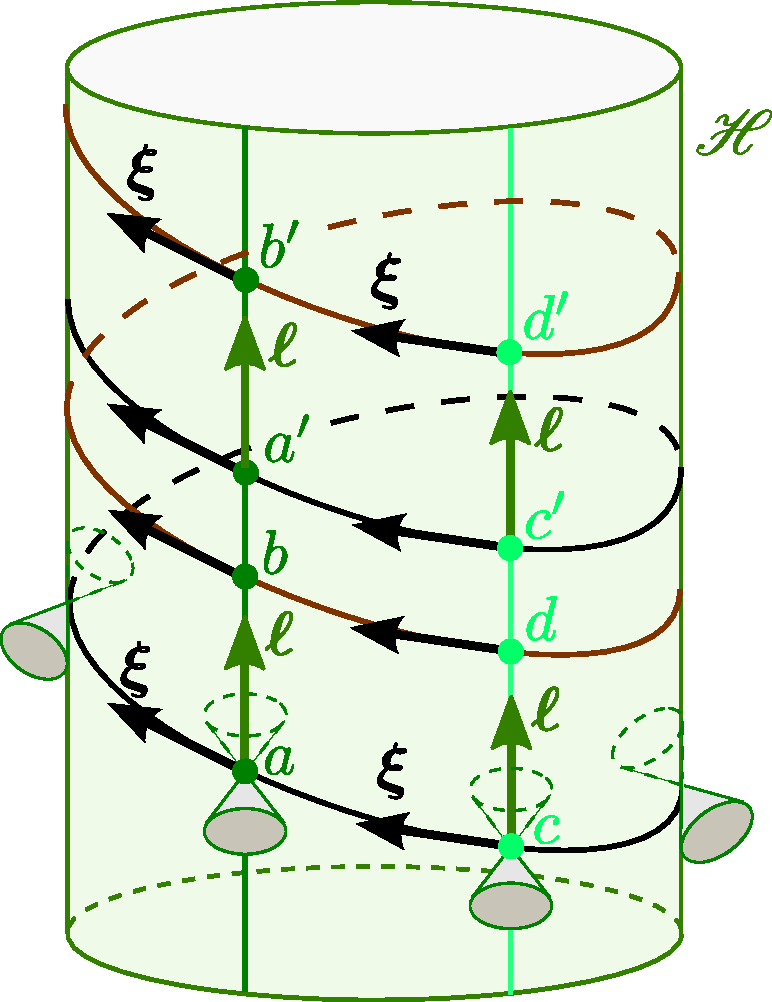
\includegraphics[height=0.4\textheight]{sta_rot_horizon_gen.pdf}
\qquad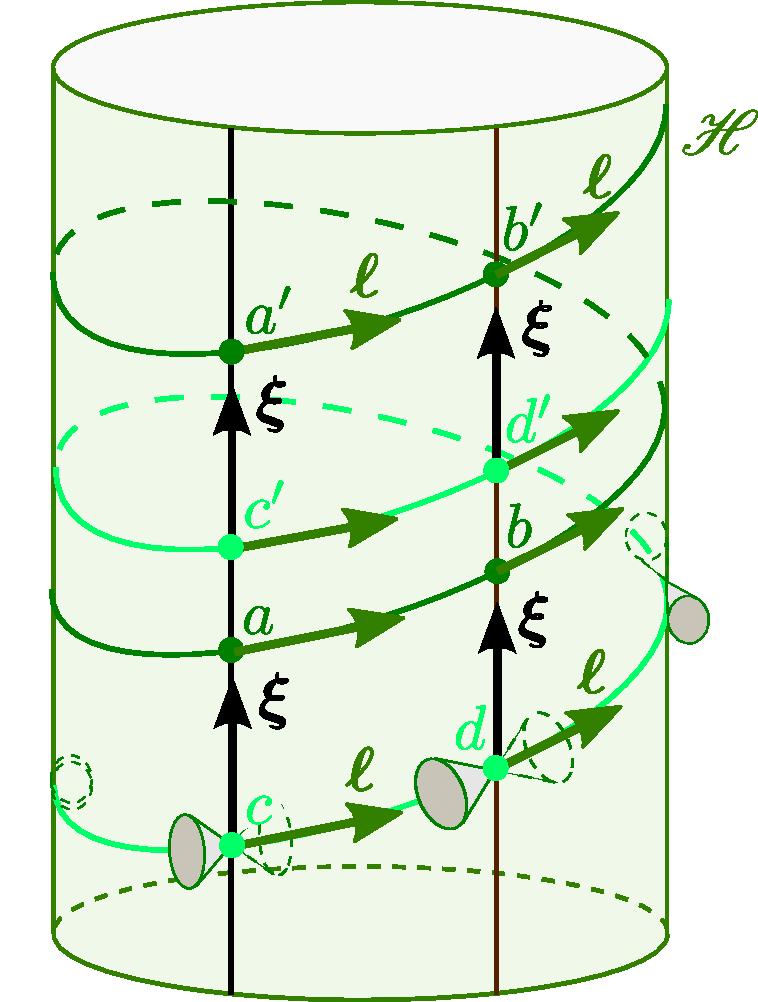
\includegraphics[height=0.4\textheight]{sta_rot_horizon_kil.pdf}}
\caption[]{\label{f:sta:rot_horizon} \footnotesize
Event horizon $\Hor$ with a stationary Killing vector field $\w{\xi}$ spacelike
on it:
\textbf{(a)} Representation with the null geodesic generators of $\Hor$ drawn as vertical
lines; two of them are actually depicted, in dark green and light green
respectively, with a null normal $\wl$ along them; besides,
two field lines of $\w{\xi}$
(orbits of the isometry group) are depicted, in black and brown
respectively.
\textbf{(b)} Representation with the field lines of $\w{\xi}$ as vertical lines.
The color code is the same as in (a) and
labelled points ($a$, $b$, etc.) help to identify
the two figures. A few light cones are drawn in each figure; note that $\w{\xi}$,
being spacelike,
is always outside of them,
while the null normal $\wl$ is always tangent to them. }
\end{figure}


\subsection{Spacelike stationary Killing field on $\Hor$: the strong rigidity theorem}
\label{s:sta:strong_rigidity}

When $\w{\xi}$ is spacelike on $\Hor$, it obviously cannot be collinear to
any null normal $\wl$ of $\Hor$.
Assuming that $\Hor$ has cross-sections of spherical topology, we observe
that, with respect to the null geodesic generators of $\Hor$, the field lines of $\w{\xi}$
form some helices, as depicted in Fig.~\ref{f:sta:rot_horizon}a. By reciprocity,
with respect to the field lines of $\w{\xi}$,
the null geodesic generators form some helices as well, as depicted in
Fig.~\ref{f:sta:rot_horizon}b):
observe that Fig.~\ref{f:sta:rot_horizon}b can be obtained from Fig.~\ref{f:sta:rot_horizon}a
by ``untwisting'' the field lines of $\w{\xi}$.

Since asymptotically the field lines of $\w{\xi}$ are worldlines of inertial observers,
Fig.~\ref{f:sta:rot_horizon}b leads us to say
(in loose terms at this stage) that the event horizon $\Hor$
``is rotating'', all the more that we have seen above that when the null
generators coincide with the field lines of $\w{\xi}$, the black hole is static, i.e. non-rotating.

Since the Killing field $\w{\xi}$ is not null on $\Hor$, we cannot say a priori
that $\Hor$ is a Killing horizon. However, modulo some additional hypotheses,
it turns out that this is the case, according to a famous result by
S.W.~Hawking\index{Hawking, S.W.} (1972)
\cite{Hawki72,HawkiE73}, known as the
\defin{strong rigidity theorem}\index{strong!rigidity theorem}\index{rigidity theorem!strong --}.
We give below a modern version of this theorem, due to Moncrief \& Isenberg
(2008) \cite{MoncrI08} (see also
Theorem~8.1 p.~470 of Choquet-Bruhat's textbook \cite{Choqu09})
\begin{prop}[strong rigidity theorem]
\label{p:sta:strong_rigidity_thm}
Let $(\M,\w{g})$ be a stationary spacetime of dimension $n\geq 4$ containing a black
hole of event horizon $\Hor$ such that the stationary Killing vector $\w{\xi}$
is spacelike on $\Hor$. If
\begin{itemize}
\item $\M$ and $\Hor$ are (real) analytic manifold
(cf. Remark~\ref{r:bas:analytic} in Sec.~\ref{s:bas:def_manif}),
with $\w{g}$ being an analytic field,
\item $\w{g}$ fulfills the vacuum Einstein equation
[Eq.~(\ref{e:fra:Einstein_eq}) with $\Lambda=0$ and $\w{T} = 0$],
\item $\Hor$ has a null geodesic generator that is incomplete,
\item $\Hor$ has compact cross-sections
\item $\w{\xi}$ is transverse to some cross-sections,
\end{itemize}
then the spacetime $(\M,\w{g})$ admits a second Killing vector field, $\w{\chi}$
say, such that
$\Hor$ is a Killing horizon with respect to $\w{\chi}$.
\end{prop}

\begin{hist}
The original version of the theorem established in 1972
by Stephen Hawking\index{Hawking, S.} \cite{Hawki72} was for a 4-dimensional
spacetime.
\end{hist}

The above theorem relies on the rather strong assumption that
the manifolds and fields are analytic.
On physical grounds,
it would be desirable to assume only \emph{smooth} manifolds and fields.
Recently, S.~Alexakis, A.D.~Ionescu and S.~Klainerman \cite{AlexaIK14} (2014)
have succeeded in proving the strong rigidity theorem without the analyticity
assumption, but only for slowly rotating black holes.

Since we have two Killing vectors, $\w{\xi}$ and $\w{\chi}$, we may
form any linear combination of them with constant coefficients
and still get a Killing vector. For instance, if $\Omega_H$ is a non-zero constant,
the vector field $\w{\eta}$ defined by
\be
    \w{\eta} = \frac{1}{\Omega_H} \left( \w{\chi} - \w{\xi} \right)
    \quad\iff\quad
    \w{\chi} = \w{\xi} + \Omega_H \w{\eta} ,
\ee
is a Killing vector field on $\M$.
One can show (see e.g. \cite{Chrus97} for a rigorous proof) that $\Omega_H$
and some constant rescaling of $\w{\chi}$
can be chosen so that $\w{\eta}$ is a spacelike vector field whose
field lines are closed, with $2\pi$-periodicity in terms of the parameter $\ph$
associated to $\w{\eta}$ (i.e. $\w{\eta} = \D/\D\ph$ along the field lines),
and such that $\w{\eta}$ vanishes on a timelike 2-dimensional surface, called
the \defin{rotation axis}\index{rotation!axis}.
It follows that
the isometry group whose generator is $\w{\eta}$ is the rotation group
$\mathrm{SO}(2)$. In other words, the spacetime $(\M,\w{g})$ is
\defin{axisymmetric}\index{axisymmetric!spacetime} in addition to being stationary.
The constant $\Omega_H$ is then called the
\defin{black hole rotation velocity}\index{black hole!rotation velocity}\index{rotation!velocity}.

By the very definition of stationarity, the Killing vector field $\w{\xi}$ is
timelike in the vicinity of $\scri^+$ and $\scri^-$. If $\w{\xi}$ is spacelike
on $\Hor$, as assumed in this section, by continuity it must be spacelike
in some part of the domain of outer communications $\langle\langle \M\rangle\rangle$
near $\Hor$. The simplest configuration is then when
$\w{\xi}$ is spacelike in some connected region $\mathscr{G}\subset \langle\langle \M\rangle\rangle$
around $\Hor$, null at the boundary of $\mathscr{G}$ and timelike outside $\mathscr{G}$
up to $\scri^+$ and $\scri^-$. The subset $\mathscr{G}$ is
called the \defin{ergoregion}\index{ergoregion} and its boundary $\E:=\partial\mathscr{G}$
the \defin{ergosphere}. We shall discuss it further in connection with
the Penrose process in Chap.~\ref{s:ker}.

%%%%%%%%%%%%%%%%%%%%%%%%%%%%%%%%%%%%%%%%%%%%%%%%%%%%%%%%%%%%%%%%%%%%%%%%%%%%%%%


\section{Bifurcate Killing horizons} \label{s:sta:bifur_Killing_hor}

Having shown that stationary black hole horizons must be Killing horizons
(Properties~\ref{p:sta:H_Killing_hor_xi_null} and \ref{p:sta:strong_rigidity_thm}),
let us move in the study of Killing horizons beyond what was achieved
in Sec.~\ref{s:neh:Killing_hor}.

\subsection{Definition and first properties} \label{s:sta:bifur_def}

\begin{greybox}
Let $(\M,\w{g})$ be a $n$-dimensional spacetime endowed with a Killing vector
field $\w{\xi}$. A
\defin{bifurcate Killing horizon}\index{bifurcate!Killing horizon}\index{Killing!horizon!bifurcate --}\index{horizon!bifurcate Killing --} is the
union
\be
    \Hor = \Hor_1 \cup \Hor_2 ,
\ee
such that
\begin{itemize}
\item $\Hor_1$ and $\Hor_2$ are two null hypersurfaces;
\item $\Sp:=\Hor_1\cap\Hor_2$ is a spacelike $(n-2)$-surface;
\item each of the sets $\Hor_1\setminus\Sp$ and $\Hor_2\setminus\Sp$ has two connected components, which are
Killing horizons\footnote{Cf. Sec.~\ref{s:neh:def_Killing_hor} for the
definition of a Killing horizon.} with respect to $\w{\xi}$.
\end{itemize}
The $(n-2)$-dimensional submanifold $\Sp$ is called the
\defin{bifurcation surface}\index{bifurcation!surface} of $\Hor$.
\end{greybox}

\begin{figure}
\centerline{\includegraphics[width=0.5\textwidth]{sta_bifur_Kill_hor.pdf}}
\caption[]{\label{f:sta:bifur_Kill_hor} \footnotesize
Bifurcate Killing horizon $\Hor_1\cup\Hor_2$ with respect to the Killing vector
field $\w{\xi}$; $\Sp$ is the bifurcation surface. $\Li_1$ and $\Li_2$ are
null geodesic generators of respectively $\Hor_1$ and $\Hor_2$, which cross
each other at the point $p\in\Sp$.}
\end{figure}

Hence we may say that a bifurcate Killing horizon is formed by four Killing horizons,
$\Hor_1^+$, $\Hor_1^-$, $\Hor_2^+$ and $\Hor_2^-$ say,
which are merged together at the bifurcation surface $\Sp$ (cf. Fig.~\ref{f:sta:bifur_Kill_hor}), in such a way that
\[
    \Hor_1 = \Hor_1^- \cup \Sp \cup \Hor_1^+ \quad \mbox{and}\quad
    \Hor_2 = \Hor_2^- \cup \Sp \cup \Hor_2^+
\]
are null hypersurfaces.

A first property of bifurcate Killing horizons is
\begin{prop}[vanishing of the Killing vector on the bifurcation surface]
\label{p:sta:xi_S_zero}
The Killing vector field vanishes on the bifurcation surface:
\be \label{e:sta:xi_S_zero}
    \encadre{\left. \w{\xi} \right| _{\Sp} = 0 } .
\ee
\end{prop}
\begin{proof}
Let $p\in \Sp$ and let us assume that $\left.\w{\xi}\right| _p\not=0$.
Let $\Li_1$ (resp. $\Li_2$) be the null geodesic generator of $\Hor_1$
(resp. $\Hor_2$) that intersects $\Sp$ at $p$ (cf. Fig.~\ref{f:sta:bifur_Kill_hor}).
Since $\Sp$ is spacelike,
$\Li_1$ and $\Li_2$ are unique. By definition of a Killing horizon,
$\w{\xi}$ is tangent to $\Li_1\cap\Hor_1^+$ and to $\Li_1\cap\Hor_1^-$,
i.e. to $\Li_1\setminus\{p\}$.
If $\left.\w{\xi}\right| _p \not=0$, then by continuity,
$\w{\xi}$ is a (non-vanishing) tangent vector field all along $\Li_1$.
Similarly, $\w{\xi}$ is tangent to all $\Li_2$.
At their intersection point $p$, the geodesics $\Li_1$ and $\Li_2$ have thus a common tangent
vector, namely $\left.\w{\xi}\right| _p$.
The geodesic uniqueness theorem (cf. Sec.~\ref{s:geo:existence_uniqueness} in Appendix~\ref{s:geo})
yields then $\Li_1 = \Li_2$.
Then $\Li_1 \subset \Hor_1 \cap \Hor_2 = \Sp$. But since $\Sp$ is spacelike and
$\Li_1$ is null, we reach a contradiction. Hence we must have
$\left.\w{\xi}\right| _p = 0$.
\end{proof}

\begin{remark}
\label{r:sta:zero_Killing}
Having a Killing vector field that vanishes somewhere (here $\Sp$) is not the sign
of any pathology: it simply means that the points of $\Sp$ are fixed points of
the isometries generated by $\w{\xi}$, since
setting $\w{\xi}=0$ in Eq.~(\ref{e:neh:xi_dxdt}) leads to $\D\w{x}=0$, i.e.
to $\Phi_{\D t}(p) = p$.
\end{remark}

\begin{remark}
Contrary to what the name may suggest, a bifurcate Killing horizon is \emph{not}
a Killing horizon, for the latter, as defined in Sec.~\ref{s:neh:def_Killing_hor},
is a regular (i.e. embedded) hypersurface
of $\M$ (cf. Sec.~\ref{s:bas:embed} in Appendix~\ref{s:bas}), while
the union of two hypersurfaces is not in general a hypersurface. Moreover
on a Killing horizon, the Killing vector field is nowhere vanishing
[cf. Eq.~(\ref{s:neh:xi_on_KH})], while on
a bifurcate Killing horizon, it is vanishing at the bifurcation surface.
\end{remark}

\begin{figure}
\centerline{\includegraphics[width=0.6\textwidth]{sta_hplane_bifur.pdf}}
\caption[]{\label{f:sta:hplane_bifur} \footnotesize
Bifurcate Killing horizon $\Hor_1\cup\Hor_2$ with respect to the Killing vector
field $\w{\xi}$ generating Lorentz boosts in the plane $(t,x)$ of Minkowski
spacetime. The dimension along $z$ having been suppressed, the bifurcation
surface $\Sp$ appears as a line, while it is actually a 2-plane.}
\end{figure}

\begin{example}[bifurcate Killing horizon w.r.t. Lorentz boost]
\label{x:sta:bif-KH-boost}
Let us consider the boost Killing vector in Minkowski spacetime as given
by Eq.~(\ref{e:neh:boost-Killing}): $\w{\xi} := x \wpar_t + t \wpar_x$
and let us take for $\Hor_1$ the null hyperplane of equation $t=x$
considered in Example~\ref{x:neh:boostKH} in Chap.~\ref{s:neh} and denoted there
by $\Hor$. The two half-hyperplanes defined by
Eq.~(\ref{e:neh:boost-Killing_hor}) are then the Killing horizons $\Hor_1^+$ and
$\Hor_1^-$. The union $\Hor_1 \cup \Hor_2$, where $\Hor_2$ is the null hyperplane of equation $t=-x$ is a bifurcate Killing horizon with respect to $\w{\xi}$,
with the 2-plane of equation $t=0$ and $x=0$ as bifurcation surface
(cf. Fig.~\ref{f:sta:hplane_bifur}). Note that on $\Hor_1$, the Killing vector
$\w{\xi}$ points away from $\Sp$, while on $\Hor_2$, it points towards $\Sp$.
\end{example}

\subsection{Non-degenerate Killing horizons and Boyer theorem}
\label{s:sta:non-degenerate_KH}

Let us consider a Killing horizon $\Hor$ with respect to some Killing vector
field $\w{\xi}$. As shown in Sec.~\ref{s:neh:zeroth_law},
modulo some mild energy condition (the null dominant energy condition),
the surface gravity\index{surface!gravity} of $\Hor$, i.e.
the non-affinity coefficient $\kappa$ of $\w{\xi}$ on $\Hor$, is constant over
$\Hor$ (the zeroth law of black hole mechanics\index{zeroth law}).
In what follows, we consider the case where $\kappa\not=0$, i.e. $\Hor$
is a non-degenerate Killing horizon (cf. Sec.~\ref{s:neh:classif_KH}).

Let us assume that $\w{\xi}$ is future-directed on $\Hor$; if not, we can
always consider $\Hor$ as a Killing horizon with respect to $-\w{\xi}$.
Let $t$ be the parameter
associated with $\w{\xi}$ along the null geodesic generators of $\Hor$, i.e.
$\w{\xi} = \D/\D t$ along any null geodesic generator $\Li$.
Since $\kappa\not=0$, $t$ is not an affine parameter of $\Li$.
The null vector field $\wl$ defined on $\Hor$ by
\be \label{e:sta:el_kappa_xi}
    \wl = \mathrm{e}^{-\kappa t} \, \w{\xi} \quad \iff\quad
    \w{\xi} = \mathrm{e}^{\kappa t} \, \wl
\ee
is a geodesic vector field and the affine parameter associated with it is
\be \label{e:sta:lambda_t}
    \lambda = \frac{\mathrm{e}^{\kappa t}}{\kappa} + \lambda_0 ,
\ee
where $\lambda_0$ is some constant.
\begin{proof}
We have
\[
\wnab_{\wl}\, \wl = \wnab_{\mathrm{e}^{-\kappa t} \w{\xi}} \left( \mathrm{e}^{-\kappa t} \, \w{\xi} \right) = \mathrm{e}^{-\kappa t} \wnab_{\w{\xi}} \left( \mathrm{e}^{-\kappa t} \, \w{\xi} \right)
= \mathrm{e}^{-\kappa t} \big[ \big( \underbrace{\wnab_{\w{\xi}} \mathrm{e}^{-\kappa t}}_{\D \mathrm{e}^{-\kappa t}/\D t} \big) \w{\xi}
    + \mathrm{e}^{-\kappa t} \underbrace{\wnab_{\w{\xi}}\, \w{\xi}}_{\kappa\w{\xi}}
    \big] = 0 .
\]
Hence $\wl$ is a geodesic vector. Besides, along any null generator of $\Hor$,
one has [cf. Eq.~(\ref{e:bas:def_vector})]
\[
    \w{\xi}(\lambda) = \frac{\D\lambda}{\D t} = \mathrm{e}^{\kappa t}
    \underbrace{\wl(\lambda)}_{1} = \mathrm{e}^{\kappa t} ,
\]
which yields Eq.~(\ref{e:sta:lambda_t}).
\end{proof}
Let us assume $\kappa>0$. Let $\Li$ be a null geodesic generator of the Killing
horizon $\Hor$. $\Li$ can be parameterized by $t$, the corresponding
tangent vector being $\w{\xi}$. When $t$ spans the whole interval $(-\infty,+\infty)$,
Eq.~(\ref{e:sta:lambda_t}) implies that $\lambda$ spans the
interval $(\lambda_0,+\infty)$ only. Since $\lambda$ is an affine parameter of $\Li$,
this means that $\Li$ is an \emph{incomplete} geodesic\index{incomplete geodesic}\index{geodesic!incomplete --} (cf. Sec.~\ref{s:geo:existence_uniqueness}).
Moreover, Eq.~(\ref{e:sta:el_kappa_xi}) leads to
\be \label{e:sta:xi_zero_t_inf}
    \w{\xi} \rightarrow 0 \quad\mbox{when}\quad t\rightarrow -\infty \qquad (\kappa>0).
\ee
In other words, the Killing vector field $\w{\xi}$ vanishes and
the null geodesic $\Li$ stops at the ``edge'' of $\Hor$ corresponding to
$t\rightarrow -\infty$.
If there is no singularity there, $\Li$ can be
extended to $\lambda\in(-\infty,\lambda_0]$, giving rise to a complete
null geodesic $\tilde\Li$. This operation can be performed for all the
null geodesic generators of $\Hor$ and we have the freedom to choose the same value
of $\lambda_0$ in Eq.~(\ref{e:sta:lambda_t}) for all of them. In this process,
one gives birth to a null hypersurface, $\tilde\Hor$ say, which contains $\Hor$. Let $\Sp\subset\tilde\Hor$ be the set of points of
affine parameter $\lambda=\lambda_0$ along all the extended null geodesics
$\tilde\Li$. $\Sp$ is clearly a cross-section of $\tilde\Hor$
(cf. Sec.~\ref{s:def:spacelike_sections}); it is then a
spacelike $(n-2)$-dimensional surface.
$\Sp$ constitutes the past boundary of $\Hor$, i.e. the boundary corresponding to $t\rightarrow -\infty$.
Since $\w{\xi}$ is a smooth vector field on $\M$, Eq.~(\ref{e:sta:xi_zero_t_inf})
implies that $\w{\xi}$ vanishes on $\Sp$.
In other words, $\Sp$ is a set of fixed points for the isometry group generated
by $\w{\xi}$ (cf. Remark~\ref{r:sta:zero_Killing} above).
Let us denote by $\Hor^-$ the subset of $\tilde\Hor$
generated by the segments $\lambda<\lambda_0$ of the null geodesics $\tilde\Li$:
$\Hor^- = \tilde\Hor\setminus(\Hor\cup\Sp)$.
$\Hor^-$ is clearly a null hypersurface.
Since $\Sp$ is spacelike and $(n-2)$-dimensional, there are, at each point
$p\in\Sp$, only two null directions normal to $\Sp$ (cf. Sec.~\ref{s:def:spacelike_sections}). One of them is along $\wl$. The set of all null geodesics
departing from $\Sp$ along the other null direction forms a null hypersurface,
$\Hor_2^+$ say, in the future of $\Sp$ and another null hypersurface, $\Hor_2^-$
say, in the past of $\Sp$.
By studying the behaviour of a Killing vector field around the set of its
fixed points (here $\Sp$), Boyer \cite{Boyer69} has shown that in
the current setting (i.e. $\Sp$ spacelike), $\w{\xi}$ acts \emph{locally}
as the generator of Lorentz boosts in Minkowski spacetime and $\Sp$ is the bifurcation surface
of a bifurcate Killing horizon similar to that of Example~\ref{x:sta:bif-KH-boost}
(cf. Fig.~\ref{f:sta:hplane_bifur}).
More precisely, Boyer proved the following theorem \cite{Boyer69}:
a Killing horizon $\Hor$ is contained in a bifurcate Killing horizon if and
only if $\Hor$ contains at least one incomplete, extendable, null geodesic
generator. The last property is guaranteed by $\kappa\not=0$, as we have seen.
It follows that $\Hor^-$, $\Hor_2^+$ and $\Hor_2^-$
are three Killing horizons, so that $\Hor\cup\Hor^-\cup\Hor_2^+\cup\Hor_2^-\cup\Sp$
is a bifurcate Killing horizon.

If $\kappa<0$, we see from Eq.~(\ref{e:sta:lambda_t}) that while $t$ spans the
whole interval $(-\infty,+\infty)$, the affine parameter $\lambda$ spans the
interval $(-\infty,\lambda_0)$ only. Moreover, Eq.~(\ref{e:sta:el_kappa_xi})
leads to
\be
    \w{\xi} \rightarrow 0 \quad\mbox{when}\quad t\rightarrow +\infty  \qquad (\kappa<0).
\ee
The reasoning developed for $\kappa>0$ can be then applied mutatis mutandis,
leading to a bifurcate Killing horizon with a bifurcation surface $\Sp$ that
is the future boundary of $\Hor$. Hence we conclude:
\begin{prop}[non-degenerate Killing horizons and bifurcate Killing horizons]
\label{p:sta:non_degen_bifurcate}
The null geodesic generators of a non-degenerate Killing horizon $\Hor$ are
incomplete; if they can be extended, $\Hor$ is contained in a
bifurcate Killing horizon, the bifurcation surface of which is the past
(resp. future) boundary of $\Hor$ if $\kappa>0$ (resp. $\kappa<0$).
\end{prop}

\begin{remark}
For a degenerate Killing horizon, the problem of extension disappears, since
$t$ is then an affine parameter of the null generators. Consequently if $t$ spans
the whole interval $(-\infty,\infty)$, the null generators are complete
geodesics. One can still have $\w{\xi}\rightarrow 0$ at some boundary
of $\Hor$, but this is a null boundary, not a spacelike one, and it does not
correspond to a bifurcation surface. An example is the Killing horizon with
respect to a null-rotation Killing vector in Minkowski spacetime, exhibited
as Examples~\ref{x:neh:nullrotKH} and \ref{x:neh:nullrotKH_kappa}
in Chap.~\ref{s:neh}, p.~\pageref{x:neh:nullrotKH} and \pageref{x:neh:nullrotKH_kappa}
respectively (cf. Fig.~\ref{f:neh:hplaneKilling-nullrot}): $\w{\xi}=0$
on the null 2-plane of equation $t=x$, $y=0$.
\end{remark}

\begin{hist} \label{h:sta:Boyer}
The concept of bifurcate Killing horizons has been introduced by Robert H. Boyer\index{Boyer, R.H.}
(1932-1966), a young American mathematical physicist just appointed to the University
of Liverpool. Sadly, Boyer was killed, among 14 victims, in a mass murder that
occurred in the University of Texas at Austin on 1 August 1966.
His last notes, containing the definition of bifurcate Killing horizon
and the proof of the above mentioned theorem, have been transformed to an article
by J. Ehlers and J.L. Stachel and published in 1969 \cite{Boyer69}.
\end{hist}

%%%%%%%%%%%%%%%%%%%%%%%%%%%%%%%%%%%%%%%%%%%%%%%%%%%%%%%%%%%%%%%%%%%%%%%%%%%%%%%

\section{The no-hair theorem} \label{s:sta:no-hair}

\subsection{Israel uniqueness theorem for static black holes}

\begin{prop}[Israel uniqueness theorem\index{Israel uniqueness theorem}]
\label{p:sta:Israel_uniqueness_thm}
If $(\M,\w{g})$ is a $n$-dimensional static spacetime
containing a black hole, with $\w{g}$ solution of the vacuum Einstein
equation, then the domain of outer communications of $\M$ is isometric
to the domain of outer communications of a $n$-dimensional Schwarzschild spacetime\index{Schwarzschild!spacetime}.
\end{prop}
This theorem has been proved in 1967 by W.~Israel \cite{Israe67},
and improved latter by many authors, in particular by
P. Chru\'sciel \& G. Galloway (2010) \cite{ChrusG10}, who removed
the hypothesis of analyticity (cf. Remark~\ref{r:bas:analytic} in Sec.~\ref{s:bas:def_manif}).
A demonstration of Israel's theorem can be found in Sec.~8.2 of
Straumann's textbook \cite{Strau13}.

So basically, in dimension $n=4$, i.e. when the staticity theorem (Property~\ref{p:sta:staticity_thm}) applies,
all stationary vacuum black holes with the stationary Killing field $\w{\xi}$ null
on $\Hor$ are nothing but Schwarzschild black holes, which we will study in detail in Chaps.~\ref{s:sch} to~\ref{s:max}.

\subsection{The no-hair theorem}

In dimension $n=4$, one can go much further then just claiming that the
event horizon of a stationary black hole must be a Killing horizon (Sec.~\ref{s:sta:EH_KH}).
One has indeed the \defin{Carter-Robinson theorem}\index{Carter-Robinson theorem}
(Carter\index{Carter, B.} 1971 \cite{Carte71}, Robinson\index{Robinson, D.C.} 1975 \cite{Robin75}):
any stationary and axisymmetric 4-dimensional asymptotically flat
black hole spacetime $(\M,\w{g})$ that is
solution of the vacuum Einstein equation with a connected regular
event horizon $\Hor$ and no closed timelike curve outside it
has a domain of outer communications that is isometric
to the domain of outer communications of the Kerr spacetime.

\begin{remark}
In their original works, Carter and Robinson assumed that $\Hor$ is a
\emph{non-degenerate}
Killing horizon, i.e. that the non-affinity coefficient $\kappa$ associated
with the Killing vector $\w{\chi}$ is non-zero (cf. Sec.~\ref{s:neh:classif_KH}). However, this non-degeneracy
hypothesis can be released \cite{ChrusN10} (see \cite{ChrusLH12} for an
extended discussion).
\end{remark}

\begin{remark}
The causality condition (absence of closed timelike curves in the black
hole exterior), which is one of the assumptions of Carter's theorem
(cf. \cite{Carte99} for a discussion), does not appear in Israel's theorem
(Property~\ref{p:sta:Israel_uniqueness_thm}) because a static spacetime, which by definition
has hypersurface-orthogonal timelike curves,
cannot contain any closed timelike curve.
\end{remark}

By combining the staticity, Israel, strong rigidity and Carter-Robinson theorems,
one arrives at the famous
\begin{prop}[no-hair theorem\index{no-hair theorem}]
Any spacetime $(\M,\w{g})$ that
\begin{itemize}
\item is 4-dimensional
\item is asymptotically flat
\item is stationary
\item is a solution of the vacuum Einstein equation
\item contains a black hole with a connected regular horizon
\item does not contain any closed timelike curve in the domain of outer
communications
\item is analytic
\end{itemize}
has a domain of outer communications that is isometric
to the domain of outer communications of the Kerr spacetime.
\end{prop}

See Ref.~\cite{IonesK15} for a review.

\begin{hist}
See the historical account by Carter \cite{Carte99}.
\end{hist}
